\documentclass[conference]{IEEEtran}
\usepackage{times}

% numbers option provides compact numerical references in the text. 
\usepackage[numbers]{natbib}
\usepackage{multicol}
\usepackage[bookmarks=true]{hyperref}

\usepackage[pdftex]{graphicx}
\usepackage{comment}

\usepackage{algorithm}
\usepackage[noend]{algpseudocode}

\usepackage{amsfonts}
\usepackage{amsmath}

\usepackage{amsthm}
\newtheorem{thm}{Theorem}
\newtheorem{lem}{Lemma}
\newtheorem{asmp}{Assumption}

\theoremstyle{definition}
\newtheorem{defn}{Definition}[section]

\pdfinfo{
   /Author (Homer Simpson)
   /Title  (Robots: Our new overlords)
   /CreationDate (D:20101201120000)
   /Subject (Robots)
   /Keywords (Robots;Overlords)
}

\begin{document}

% paper title
\title{ MORRF$^{*}$ : Sampling-Based Multi-Objective Motion Planning }

% You will get a Paper-ID when submitting a pdf file to the conference system
\author{Author Names Omitted for Anonymous Review. Paper-ID [add your ID here]}

\maketitle

\begin{abstract}
The importance of multi-objective path planning emerges with the increase of the requirement complexity of the robot's tasks.
The nature of the path planning problem makes that a few of the multi-objective optimization methods could not be directly imported to find the Pareto optimal solutions.
Inspired by the RRT* and the decomposition-based multi-objective optimization, we proposed a MORRF*(Multi-objective Rapidly exploring Random Forest*) in this paper that could effectively and efficiently find the Pareto optimal set of solutions.
The RRF consists of two types of tree structures, the reference tree and the subproblem tree.
Each reference tree explores a single objective to support the estimation of an Utopia position in the fitness space.
Each subproblem tree explores to find a solution to the assigned subproblem.
The solutions from all the trees form a set of Pareto optimal solutions. 

Theoretical analysis has been shown to support the feasibility of this algorithm and the asymptotic optimality. 
Simulations have been take to show the effectiveness and the efficiency of the MORRF*.
\end{abstract}

\IEEEpeerreviewmaketitle

\begin{comment}
Final Paper Submission Deadline: January 22, 2015, 23:59 PST

Papers can be up to 8 pages + references. 
This means that if more than 8 pages are used, the 9th and subsequent pages should contain ONLY references. 
The length requirement will be strictly enforced.
\end{comment}

\begin{comment}


\end{comment}

\section{Introduction}
\label{sec:intro}

\begin{comment}
(1) Why the multi-objective path planning is needed 
(2) Why the multi-objective path planning is hard (compare with a common multi-objective optimization problem)
\end{comment}

In many real applications of the robots, the complexity of tasks inherently implies more than single objective to be reached.
A robot in a search task is usually expected to maximize the search coverage with a consideration of the energy efficiency so that the execution time could also be expanded~\cite{yi2014supporting}. 
If there exists risk in the working environment, the robot should also try to avoid dangerous regions.
In robot arm manipulation planning, there usually exist several criteria to be considered as well~\cite{Pires2004}, for example, movement, joint velocities, joint accelerations and etc. 
The multiple objectives in a planning optimization are usually incomparable and conflicted.
When those objectives could not be converted into single measurable objective, the multi-objective optimization will be needed to find a set of non-dominant solutions.
A non-dominant solution means that there exists no other solution can surpass it in all the objectives.
In optimal design, a human interactive process can help the decision maker finding the most preferred solution, especially when the decision maker's preference is hard to precisely describe.

Finding Pareto optimal solutions in the multi-objective optimal path planning is much more difficult.
The popular methods in multi-objective optimization cannot be directly applied to a path planning problem.
One way is coding a path into a fixed-length solution by direction~\cite{Ahmed2013} or way points~\cite{5160222}.
Evolutionary algorithms could then be imported to search the optimal solutions.
In order to have a better approximation, the number of the segments consisted of a path cannot be too small.
This will make the solutions in a rather high dimension solution space.
However, representing the path trajectory by fixed number of segments might lead to problems in complex environment.
With different shapes and sizes of obstacles, it is hard to estimate how many segments would be enough to represent all the possible paths.
Allowing different segment numbers of the paths could help but the solution format won't fit the requirement of most of the evolutionary algorithms.
Also, when modeling a path into a point in a solution space, the obstacles in the working space could make a few of infeasible regions, which influences the continuity and increases the hardness of the heuristic-based search~\cite{5160222}~\cite{4358754}.

RRT(Rapidly exploring Random Tree) is a popular algorithm in finding feasible solutions from a start position to a goal position, which supports well in the environments with complex obstacles. 
The tree structure also guarantees a great efficiency on path search.
RRT* was recently introduced and has been proven to effectively finding an optimal path given enough sampling time~\cite{Karaman:2011:SAO:2000201.2000209}~\cite{Karaman.Frazzoli:RSS10}.
Similar with that decomposing the multi-objective optimization problem into a few subproblems in \cite{4358754}, we propose the MORRF*(Multi-Objective Rapidly exploring Random Forest*) to find a set of Pareto optimal paths from the start position to the goal position.

In this paper, we reviews a few existing multi-objective path planning algorithms and the works that inspires our algorithm in Section \ref{sec:related_works}.
With the definition of the multi-objective path planning problem, MORRF* is introduced and explained in Section \ref{sec:morrt}.
We provide theoretic analysis to support MORRF* in Section \ref{sec:theoretic_analysis}.
Simulation results are given in Section \ref{sec:simulation} to illustrate the performance of the proposed algorithm.

\section{Related works}
\label{sec:related_works}

Finding a set of Pareto optimal paths replies on exploring the non-dominance of the paths.
The implicit comparative property prevents a few pruning techniques for efficiency and the algorithm complexity would be greatly extended.
By modeling the working space into the connectivity of a graph structure, a multi-objective A* search could be applied to find the solution set in \cite{Mandow:2005:NAM:1642293.1642328}.
In a grid map, the paths could be coded into a sequence of directions from one cell to next cell.
NSGA-II can then be used to find a set of Pareto optimal solutions in \cite{Ahmed2013}.
The solutions would be obtained as sequences of way points.
To better support the environment with obstacles, spline are introduced to interpolate a sequence of way points into a trajectory in \cite{6181426}.
It reveals the drawbacks of this format of path trajectory. 
This process might also deviate the path from the found optimal result.
Increasing the path resolution, the number of the steps, should better deal with the obstacles in the working space and also follows better along the gradient of the fitness.
But the dimension of the solution space would be increased.
As a result, the search time could be significantly expanded.
The exist of obstacles also make plenty of paths infeasible.
This leads to the discontinuity of the solution space, which could impact the performance of many evolutionary algorithm on multi-objective optimization.

The discretized map only approximates the environment, which might lose a lot of environmental information.
Some of the obstacles' shapes could not be well considered in the planning process.

If we model the problem in a continuous space, the solution space is greatly expanded. 
It will take much longer time to converge to the Pareto front.
RRT(Rapidly exploring random tree) has been a popular tool to path planning in a continuous space.
It efficiently explores the space by randomly sampling and works well with any complex obstacles.
The simplicity of the algorithm ensures the search time of a feasible solution can be very short.
It is figured out that RRT fails to find an optimal solution in the optimal path planning in \cite{Karaman.Frazzoli:RSS10}.
RRT* is introduced to facilitate the optimal search.
A \emph{Rewire} process is imported to update the tree structure towards optimality.
It has been proven that RRT* shows asymptotic optimality.
It actually learns the optimal path from each vertex of the tree structure to the start position.
Figure \ref{fig:RRTstar2} gives an example.
\begin{figure}
\centering
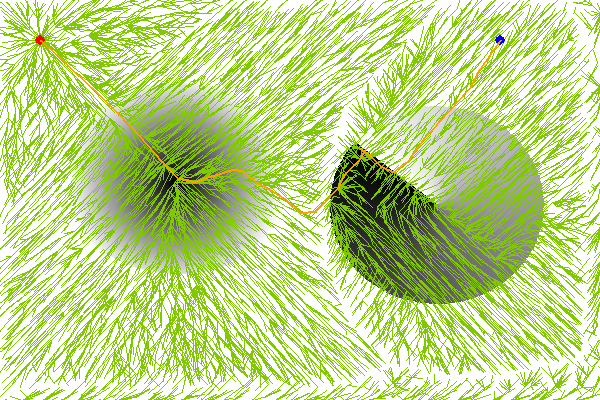
\includegraphics[width=0.7\linewidth]{fig/RRTstar2}
\caption{Tree structure after exploring fitness space.}
\label{fig:RRTstar2}
\end{figure}

Besides dominance comparison, decomposition is another effective way to find Pareto optimality.
MOEA-D is proposed in \cite{4358754}, which decomposes a multi-objective optimization problem into a class of subproblems.

Let $ \vec{\lambda} = [ \lambda_{1} , \cdots , \lambda_{K}  ]^{T} $ be a weight vector and $ \sum_{k=1}^{K} \lambda_{k} = 1 $.
Three types of decomposition methods are introduced in \cite{4358754}.
\begin{itemize}
\item \emph{Weighted sum approach} \\
Maximize $ g^{ws} (x \mid \vec{\lambda}) = \sum_{k=1}^{K} \lambda_{k} f_{k} (x) $;
\item \emph{Tchebycheff approach} \\
Minimize $ g^{te} (x \mid \lambda , z^{*}) = \max_{i \leq k \leq K}  \{ \lambda_{i} | f_{k}(x) - z^{*}_{k}  | \} $;
\item \emph{Boundary intersection approach} \\
Minimize $ g^{bi} (x \mid \lambda , z^{*} ) = d $, subject to $ z^{*} - F(x) = d \lambda $.
\end{itemize}
A few evolutionary algorithms based on the decomposition are proposed to solve the multi-objective optimization~\cite{6600851}, 
especially in many-objective optimization problems.
It is noticeable that the decomposition depends on finding the ``Utopia'' point as a reference to minimize different weighted distances.
In the next section, we will propose an algorithm that explores the solution spaces parallel using an RRT* tree structure.



\section{Multi-Objective Rapidly exploring Random Forest$^{*}$}
\label{sec:morrt}

The multi-objective path planning problem is usually defined as:
\begin{defn}{ \textbf{Multi-Objective Path Planning} }
	Given a bounded connect open set $ X \subset \mathbb{R}^{d} $, an obstacle space $ X_{obs} $, an initial state $ x_{init} $, and a goal region $ X_{goal} $.
	Given $ K $ objectives that are determined by a vector function
	$ \vec{F}(x) = [ f_{1} (x), \cdots , f_{K}(x) ]^{T} : \mathbb{R}^{d} \rightarrow \mathbb{R}^{K} $ and 
	$ \vec{F}(\sigma) = \sum_{x \in \sigma} \vec{F}(x) $.
	Find paths $ \sigma^{*} \in \Sigma^{*}  : [0, s] \rightarrow cl(  X \setminus X_{obs} ) $ such that
	\begin{itemize}
		\item $ \sigma^{*} (0) = x_{init} $ and $ \sigma^{*} (s) = X_{goal}  $;
		\item $ \not \exists \sigma , \forall k \in K, f_{k} (\sigma) > f_{k} (\sigma^{*}) $.
	\end{itemize}
\end{defn}

The solution set will be obtained by decomposing it into $ N $ subproblems.

There are two types of tree structures used for the optimization process.
\begin{itemize}
\item Each \emph{reference tree} explores for a single objective $ f_{k} (x), k \in K $. 
\item Each \emph{subproblem tree} explores for a subproblem $ g_{m} ( x \mid \lambda_{m} , z^{*} ) , m \in M $.
\end{itemize}
The paths found from both the subproblem trees and the reference trees consist of the solution set.


Because the convergence of the tree structure in RRT* means that the path from the root to any vertex is an optimal path of the defined cost.
We use the same sampling position to extend all the trees in one iteration.
Thus the vertices in the reference trees could be used as reference for estimating the cost in constructing the subproblem trees.

Like all the sampling-based optimization, the random positions are uniformly sampled from the workspace.
It means that all the tree have equivalent vertices constructed from same positions set sequentially.
But they are connected by different measurements of the costs, either a single objective or a cost from subproblem definition.
The edges of the trees can be different.

\begin{figure}[H]
\centering
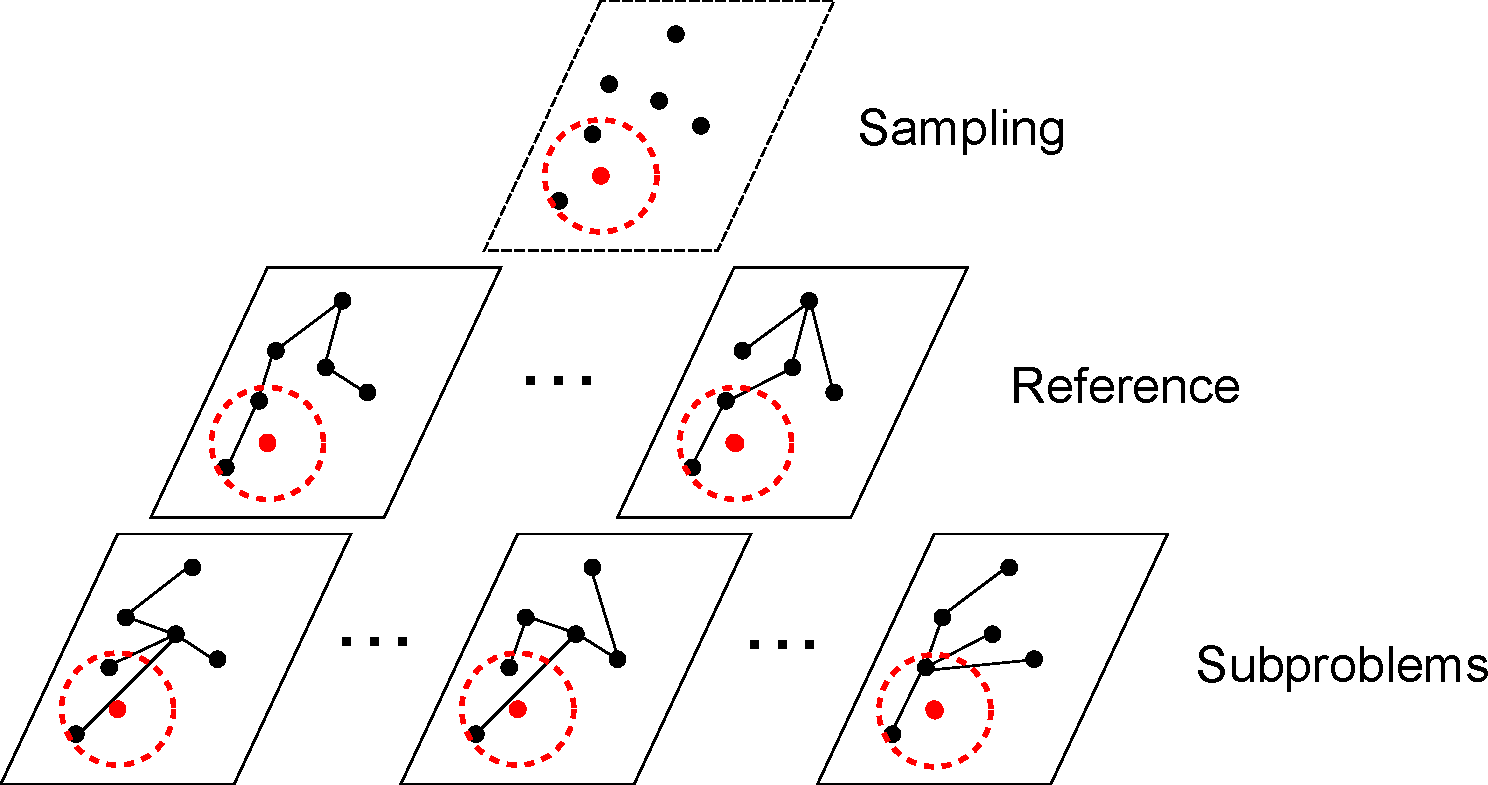
\includegraphics[width=0.9\linewidth]{./fig/MORRTstar}
\caption{Rapidly Exploring Process}
\label{fig:MORRTstar}
\end{figure}


\begin{algorithm}
\begin{algorithmic}[1]
\For{ \textbf{each} $ V_{r} \in \mathbf{V}_{r} $ } 
	\State $ V_{r} \leftarrow \{ x_{init} \} $; $ E_{r} \leftarrow \emptyset $; $ i \leftarrow 0 $
\EndFor
\For{ \textbf{each} $ V_{s} \in \mathbf{V}_{s} $ } 
	\State $ V_{s} \leftarrow \{ x_{init} \} $; $ E_{s} \leftarrow \emptyset $; $ i \leftarrow 0 $
\EndFor
\While{ $ i < N $ }
	\For{ \textbf{each} $ G_{r} \in \mathbf{G}_{r} $ } 
		\State $ G_{r} \leftarrow (V_{r}, E_{r}) $
	\EndFor
	\For{ \textbf{each} $ G_{s} \in \mathbf{G}_{s} $ } 
		\State $ G_{s} \leftarrow (V_{s}, E_{s}) $
	\EndFor
	\State $ x_{rand} \leftarrow $ \Call{ Sample }{$ i $} ; $ i \leftarrow i + 1 $
	\State $ V' \leftarrow V $; $ E' \leftarrow E $
	\State $ x_{nearest} \leftarrow $ \Call{Nearest}{$ G, x $}
	\State $ x_{new} \leftarrow $ \Call{Steer}{$ x_{nearest}, x $}
	\If{ \Call{ObstacleFree}{$ x_{nearest}, x_{new} $} }
		\For{ \textbf{each} $ G_{r} \in \mathbf{G}_{r} $ } 
		\State $ (V_{r}, E_{r}) \leftarrow $ \Call{ Extend$_{Ref}$ }{$ G_{r}, x_{new} $}
		\EndFor
		\For{ \textbf{each} $ G_{s} \in \mathbf{G}_{s} $ } 
		\State $ (V_{s}, E_{s}) \leftarrow $ \Call{ Extend$_{Sub}$ }{$ G_{s}, x_{new} $}
		\EndFor
	\EndIf
\EndWhile
\end{algorithmic}
\label{alg:rapidly_exploring_process}
\caption{Multi-objective Rapidly Random exploring }
\end{algorithm}

\begin{algorithm}
\begin{algorithmic}[1]
\State $ V' \leftarrow V' \cup \{ x_{new} \} $
\State $ x_{min} \leftarrow x_{nearest} $
\State $ X_{near} \leftarrow $ \Call{Near}{$ G, x_{new}, | V | $}
\For{\textbf{each} $ x_{near} \in X_{near} $ }
	\If{ \Call{ObstacleFree}{$ x_{new} , x_{near} $} }
		\State $ c_{k}' \leftarrow $ \Call{Cost$_{k}$}{$ x_{near} $} $ + c_{k}( $ \Call{Line}{$ x_{near}, x_{new} $} $ ) $ 
		\If{ $ c_{k}' < $ \Call{Cost$_{k}$}{$ x_{new} $} }
		\State $ x_{min} \leftarrow x_{near} $
		\EndIf
	\EndIf
\EndFor
\State $ E' \leftarrow E' \cup \{ ( x_{min}, x_{new} ) \} $
\For{\textbf{each} $ x_{near} \in X_{near} \setminus \{ x_{min} \} $ }
	\If{\Call{ObstacleFree}{$ x_{new} , x_{near} $}}
	    \State $ c_{k}' \leftarrow $ \Call{Cost$_{k}$}{$ x_{new} $} $ + c_{k}( $ \Call{Line}{$ x_{new}, x_{near} $} $ ) $ 
	    \If{ $ c_{k}' < $ \Call{Cost$_{k}$}{$ x_{near} $} }
			\State $ x_{parent} \leftarrow $ \Call{Parent}{$ x_{near} $}
			\State $ E' \leftarrow E' \setminus \{ ( x_{parent}, x_{near} ) \} $
			\State $ E' \leftarrow E' \cup \{ ( x_{new}, x_{near} ) \} $
		\EndIf
	\EndIf
\EndFor
\Return $ G' = (V', E') $ 
\end{algorithmic}
\label{alg:morrtstar:extend:ref}
\caption{ $ \mbox{Extend}_{Ref} (G, x) $}
\end{algorithm} 

\begin{algorithm}
\begin{algorithmic}[1]
\State $ V' \leftarrow V' \cup \{ x_{new} \} $
\State $ x_{min} \leftarrow x_{nearest} $
\State $ X_{near} \leftarrow $ \Call{Near}{$ G, x_{new}, | V | $}
\For{\textbf{each} $ x_{near} \in X_{near} $ }
	\If{ \Call{ObstacleFree}{$ x_{new} , x_{near} $} }
		\State $ \vec{c}' \leftarrow $ \Call{Cost}{$ x_{near} $} $ + \vec{c}( $ \Call{Line}{$ x_{near}, x_{new} $} $ ) $ 
		\State $ \eta' =  $ \Call{Fitness}{ $ \vec{c}' , \vec{c}^{*} \mid \lambda_{G} $ }
		\State $ \vec{c}_{new} = $ \Call{Cost}{$ x_{new} $} 
		\State $ \eta_{new} = $ \Call{Fitness}{ $ \vec{c}_{new} , \vec{c}^{*} \mid \lambda_{G} $ }
		\If{ $ \eta' < \eta_{new} $ }
			\State $ x_{min} \leftarrow x_{near} $
		\EndIf
	\EndIf
\EndFor
\State $ E' \leftarrow E' \cup \{ ( x_{min}, x_{new} ) \} $
\For{\textbf{each} $ x_{near} \in X_{near} \setminus \{ x_{min} \} $ }
	\If{\Call{ObstacleFree}{$ x_{new} , x_{near} $} }
		\State $ \vec{c}' \leftarrow $ \Call{Cost}{$ x_{new} $} $ + \vec{c}( $ \Call{Line}{$ x_{new}, x_{near} $} $ ) $ 
		\State $ \eta' =  $ \Call{Fitness}{ $ \vec{c}' , \vec{c}^{*} \mid \lambda_{G} $ }
		\State $ \vec{c}_{near} = $ \Call{Cost}{$ x_{near} $} 
		\State $ \eta_{near} = $ \Call{Fitness}{ $ \vec{c}_{near} , \vec{c}^{*} \mid \lambda_{G} $ }
		\If{ $ \eta' < \eta_{near} $ }
			\State $ x_{parent} \leftarrow $ \Call{Parent}{$ x_{near} $}
			\State $ E' \leftarrow E' \setminus \{ ( x_{parent}, x_{near} ) \} $
			\State $ E' \leftarrow E' \cup \{ ( x_{new}, x_{near} ) \} $
		\EndIf
	\EndIf
\EndFor
\Return $ G' = (V', E') $ 
\end{algorithmic}
\label{alg:morrtstar:extend:sub}
\caption{ $ \mbox{Extend}_{Sub} (G, x) $}
\end{algorithm} 


\section{Theoretic Analysis}
\label{sec:theoretic_analysis}

Several assumptions are needed, which are inherited from RRT$^{*}$~\cite{Karaman.Frazzoli:RSS10}.
\begin{asmp}{(Additivity of the objective functions)}
For all $ k \in K $, $ \sigma_{1} , \sigma_{2} \in X \setminus X_{obs} $,
$ c_{k} ( \sigma_{1}  \mid \sigma_{2} ) = c_{k} ( \sigma_{1} ) + c_{k} ( \sigma_{2} ) $.
\end{asmp}

\begin{asmp}{(Continuity of the objective functions)}
For all $ k \in K $, the cost function $ c_{k} $ is Lipschitz continuous,
$ \forall \sigma_{1} : [ 0, s_{1} ] \rightarrow X \setminus X_{obs}, \sigma_{2} : [0, s_{2} ] \rightarrow X \setminus X_{obs} $,
$ \exists k $ such that 
$ | c_{k} ( \sigma_{1} ) - c_{k} ( \sigma_{2} ) | \leq k \sup_{\tau \in [0,1]} \lVert \sigma_{1} (\tau s_{1}) - \sigma_{2} (\tau s_{2}) \rVert $
\end{asmp}

\begin{asmp}{(Obstacle spacing)}
There exists a constant $ \delta \in \mathbb{R}_{+} $ such that $ \forall x \in X \setminus X_{obs} $ , $ \exists x' \in X \setminus X_{obs} $ such that
\begin{itemize}
\item the $ \delta $-ball centered at $ x' $ lies inside $ X \setminus X_{obs} $;
\item $ x $ lies inside the $ \delta $-ball centered at $ x' $.
\end{itemize}
\end{asmp}

\begin{lem}
\label{lem:moo-d:rrt}
The decomposition method is applicable to the sampling-based path planning.
\begin{proof}
In a sampling-based path planning problem, let $ N_{i} $ be the number of samplings at iteration $ i $.
In the cost minimization problem, assume there is no loop in a path, which means that a path will not visit a visited vertex.
As a path $ \sigma $ is a sequence of vertices, the maximum size of a path is less than $ N_{i} $, i.e.
$ | \sigma | \leq N_{i} $.
Let $ \bar{i} $ be the stopping iteration number.
The number of vertices in any path is less than $ N_{ \bar{i} } $, which can be represented as a path of length $ N_{ \bar{i} } $ by duplicating the vertices in a path.
For example, duplicating $ x_{2} $ in $ (x_{1} , x_{2}, x_{3} ) $ makes an equivalent path of length $ 4 $ , $ (x_{1} , x_{2},  x_{2}, x_{3} ) $.
The cost will not be changed, $ f( (x_{1} , x_{2}, x_{3}) ) = f( (x_{1} , x_{2},  x_{2}, x_{3} ) )$.
Using a space of dimension $ N_{ \bar{i} } $, any path $ \sigma $ in a sampling-based path planning problem can be mapped into a point in the same space.
The decomposition methods mentioned in \cite{4358754} can be imported in this case.		
\end{proof}
\end{lem}

\begin{figure}
\centering
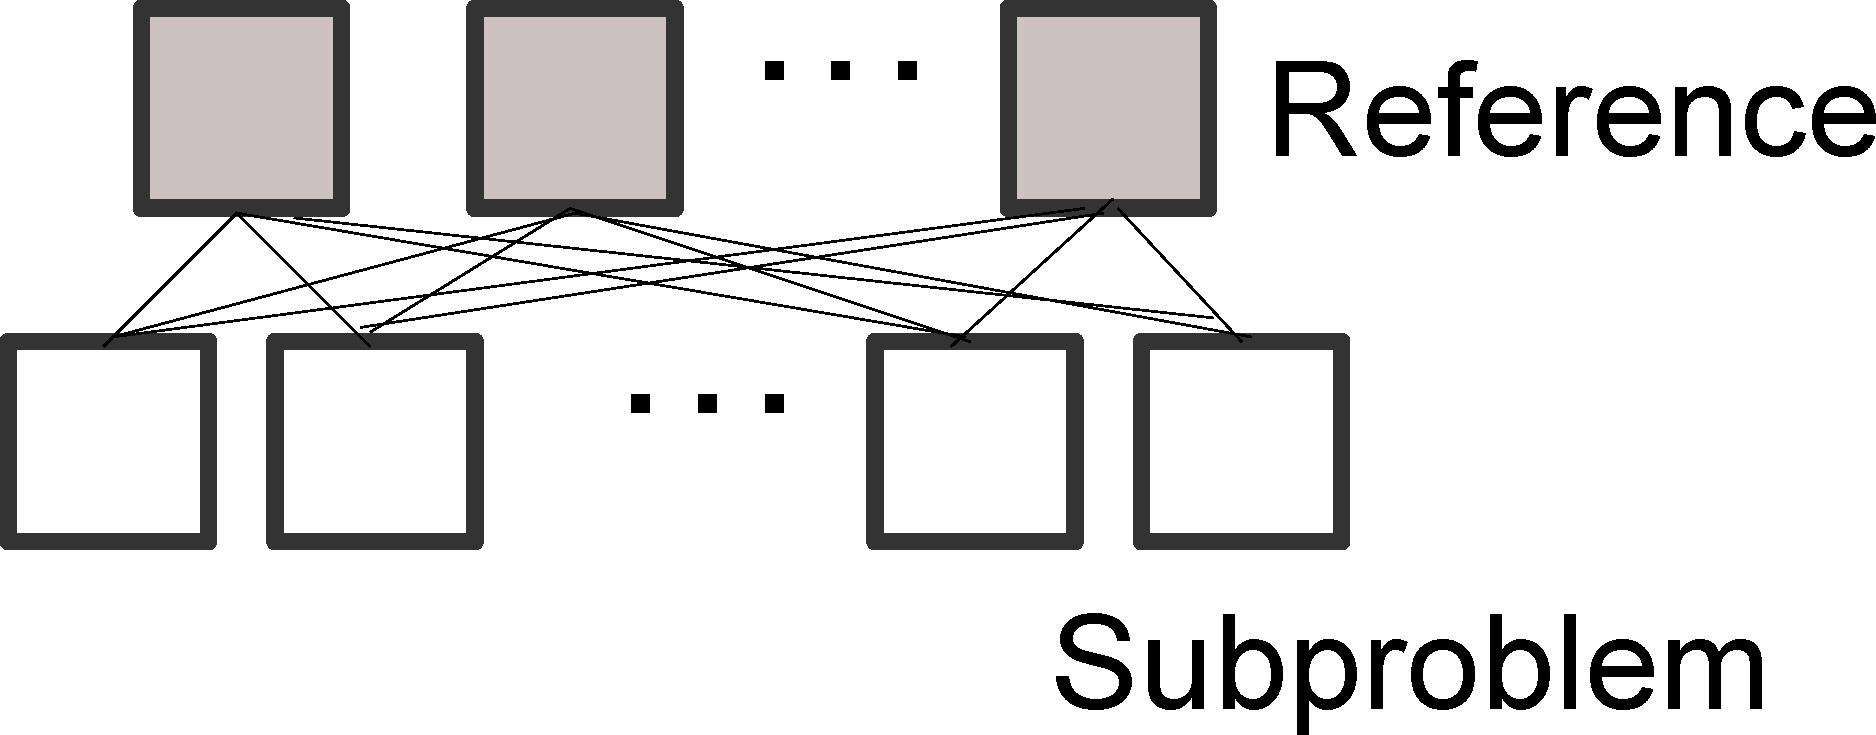
\includegraphics[width=0.7\linewidth]{fig/dependency}
\caption{The dependency of the trees in MORRF$^{*}$.}
\label{fig:dependency}
\end{figure}


\begin{lem}
\label{lem:ref_tree:conv}
The cost of the solution of $ k $-th reference tree converges to $ z^{*}_{k} $, i.e., 
$ P( \{ \lim_{ i \rightarrow \infty }  c_{k} ( i ) = z^{*}_{k}  \} ) = 1  $.
\begin{proof}
The construction of a reference tree does not depend on any other tree.
The construction process is equivalent to the construction of a RRT*.
The asymptotic optimality of RRT* is inherited here.
Thus the cost of the solution converges to the optimal of one single objective.
\end{proof}
\end{lem}

\begin{lem}
\label{lem:tree_vex:conv}
The cost of the minimum cost path from the root to any vertex in RRT$^{*}$ converges to the optimal cost almost surely, i.e.,
$
P( \{ \lim_{ i \rightarrow \infty } c(x, i)  = z^{*}(x) \} ) = 1, x \in V $.
\begin{proof}
The construction of RRT* is not goal-oriented.
The ``rewire'' process potentially will update all the vertices and converge the value to the optimal one.
Similar with that of a goal vertex, the paths from the root to all other vertices will converge to corresponding optimal ones as well.
\end{proof}
\end{lem}

\begin{lem}
\label{lem:sub_tree:conv}
The cost of the solution of $ m $-th subproblem tree converges to the optimal cost of the $ m $-th subproblem, i.e.,
$
P( \{ \lim_{ i \rightarrow \infty } c_{ \lambda_{m} }( i ) \} ) = z^{*}_{ \lambda_{m} }
$
\begin{proof}
The construction of a subproblem tree depends on the convergence of all the reference trees.
When all the reference trees have converged, the correct reference values $ c^{*} (x) $ of all the vertices could be obtained.
The convergence process will be similar with that of a single RRT*.
By Lemma \ref{lem:ref_tree:conv} and Lemma \ref{lem:sub_tree:conv}, we know that the utopia reference value $ c^{*} (x) $ could be correctly estimated after all the reference trees have reached optimality.
\end{proof}
\end{lem}

\begin{thm}
\label{thm:morrt:conv}
The solutions from MORRF$^{*} $ converges to the Pareto optimal set almost surely, i.e.
$
P( \lim_{ i \rightarrow \infty }  \Sigma^{\mbox{MORRF}^{*}}_{i}  \subset \Sigma^{*} ) = 1.
$
\begin{proof}
\end{proof}
\end{thm}

\section{Simulation}
\label{sec:simulation}

\begin{comment}
2D (weighted sum + Tchebycheff method)
2D (With obstacles)
3D
compare NSGA-II
\end{comment}

Simulations have been taken to verify the performance of MORRF$^{*}$.
We 
We also implemented NSGA-II for multi-objective path planning, which is introduced in \cite{Ahmed2013}.
In order to be comparable, the path planning using NSGA-II is implemented in a continuous space.
Each solution is represented as a sequence of way points.
The cost is calculated like that in RRT*, whcih \textsc{Line}($ x_{1}, x_{2} $) is called to calculate the cost between two way points $ x_{1} $ and $ x_{2} $.


We tested firstly on path planning of two objectives.





\section{Conclusion} 
\label{sec:conclusion}

The conclusion goes here.

\section*{Acknowledgments}

%% Use plainnat to work nicely with natbib. 

\bibliographystyle{plainnat}
\bibliography{reference}

\end{document}